\documentclass[11pt]{beamer}
\usetheme{Madrid}
\usepackage[utf8]{inputenc}

\usepackage{hyperref}
\usepackage{amsmath}
\usepackage{amsfonts}
\usepackage{amssymb}
\usepackage{graphicx}
\DeclareMathOperator{\argmin}{argmin}
\usepackage{algorithmic}
\usepackage{algorithm}
\usepackage{wrapfig}
\usepackage{subcaption}
\graphicspath{{.}}

\author{Generic Name}
\title{Title for Super Fancy Stuff}
% Informe o seu email de contato no comando a seguir
% Por exemplo, alcebiades.col@ufes.br
\newcommand{\email}{lalala@lala.la}
\setbeamercovered{transparent}
\setbeamertemplate{navigation symbols}{}
%\logo{}
\institute[]{Some Super Fancy Institution}
\date{\today}
\subject{Subject Title }

% ---------------------------------------------------------
% Selecione um estilo de referência
\bibliographystyle{IEEEtran}

%\bibliographystyle{abbrv}
%\setbeamertemplate{bibliography item}{\insertbiblabel}
% ---------------------------------------------------------

% ---------------------------------------------------------
\newtheorem{remark}{Remark}
\newtheorem{assumption}{Assumption}

\begin{document}

\begin{frame}
    \titlepage
\end{frame}

\begin{frame}{ToC}
    \tableofcontents
\end{frame}

\section{This is the First Section}
    \subsection{Taxonomy of Proximal type of Methods}
        \begin{frame}{Frame Title}
            
            \begin{block}{Formula Presented in Block}
                \begin{align}
                    \min_{x} g(x) + h(x)
                \end{align}    
            \end{block}
            
            \begin{itemize}
                \item [1.]Throughout this presentation, we assume the objective of a function $f$ is the sum of 2 functions.
                \item [2.]We are interested in the paper: FISTA (Fast Iterative-Shrinkage Algorithm) by Beck and Teboulle \cite{paper:FISTA}. 
                \pause 
                \item [1.] When $h = \delta_Q$ with $Q$ closed and convex with $Q\subseteq \text{ri}\circ \text{dom}(g)$, we use projected subgradient. 
                \item [2.] When $g$ is \textbf{\emph{strongly smooth}} and $h$ is \textbf{closed convex proper} whose proximal oracle is easy to compute, we consider the use of FISTA. 
            \end{itemize}
                
        \end{frame}
        
    \subsection{The Proximal Operator}
        \begin{frame}{Frame Title}
            \begin{definition}[Definition of Something]
                Let $f$ be convex closed and proper, then the proximal operator parameterized by $\alpha > 0$ is a non-expansive mapping defined as: 
                \begin{align*}
                    \text{prox}_{f, \alpha}(x) := 
                    \arg\min_{y}\left\lbrace
                        f(y) + \frac{1}{2\alpha} \Vert y - x\Vert^2
                    \right\rbrace. 
                \end{align*}
            \end{definition}  
            \begin{remark}
                When $f$ is convex, closed, and proper, 
            \end{remark}
        \end{frame}

        \begin{frame}{Prox is the Resolvant of Subgradient}
            \begin{lemma}[The Lemma]\label{lemma:prox_alternative_form}
                When the function $f$ is convex closed and proper, the $\text{prox}_{\alpha, f}$ can be viewed as the following operator $(I + \alpha \partial f)^{-1}$. 
            \end{lemma}
            \begin{proof}
                Minimizer satisfies zero subgradient condition, 
                {\scriptsize
                \begin{align*}
                    \mathbf 0 &\in \partial
                    \left[
                        \left.
                            f(y) + \frac{1}{2\alpha} \Vert y - x\Vert^2 
                        \right| y
                    \right](y^+)
                    \\
                    \mathbf 0 &\in \partial f(y^+) + \frac{1}{\alpha}(y^+ - x)
                    \\
                    \frac{x}{\alpha} &\in 
                    (\partial f + \alpha^{-1}I)(y^+)
                    \\
                    x &\in 
                    (\alpha \partial f + I)(y^+)
                    \\
                    y &\in (\alpha\partial f+ I)^{-1}(x).
                \end{align*}
                }
            \end{proof}
                
        \end{frame}
        
        
    \subsection{Strong Smoothness}
        \begin{frame}{Equivalence of Strong Smoothness and Lipschitz Gradient}
            \begin{theorem}[Lipschitz Gradient Equivalence under Convexity]
                Suppose $g$ is differentiable on the entire of $\mathbb E$. It is closed convex proper. It is strongly smooth with parameter $\alpha$ if and only if the gradient $\nabla g$ is globally Lipschitz continuous with a parameter of $\alpha$ and $g$ is closed and convex. 
                \begin{align*}
                    \Vert \nabla g(x) -\nabla g(y)\Vert \le 
                    \alpha 
                    \Vert x - y \Vert\quad \forall x, y\in \mathbb E
                \end{align*}
            \end{theorem}
            \begin{proof}
                Using line integral, we can prove Lipschitz gradient implies strong smoothness without convexity. The converse requires convexity and applying generalized Cauchy Inequality to (iv) in Theorem 5.8 for Beck's textbook \cite{book:first_order_opt}. 
            \end{proof}
            
        \end{frame}
    \subsection{A Major Assumption}    
        \begin{frame}{A Major Assumption}
            \begin{assumption}[Convex Smooth Nonsmooth with Bounded Minimizers]\label{assumption:1}
                We will assume that $g:\mathbb E\mapsto \mathbb R$ is \textbf{strongly smooth} with constant $L_g$ and $h:\mathbb E \mapsto \bar{\mathbb R}$ \textbf{is closed convex and proper}. We define $f := g + h$ to be the summed function and $\text{ri}\circ \text{dom}(g) \cap \text{ri}\circ \text{dom}(h) \neq \emptyset$. We also assume that a set of minimizers exists for the function $f$ and that the set is bounded. Denote the minimizer using $\bar x$. 
            \end{assumption}
        \end{frame}
        
    
\section{A New Fancy Section}
    \subsection{A Fancy Subsetction for Algorithm}
        \begin{frame}{The Accelerated Proximal Gradient Method}
            \begin{block}{Momentum Template Method}
                \begin{algorithm}[H]
                    \begin{algorithmic}[1]
                        \STATE{\textbf{Input:} $x^{(0)}, x^{(-1)}, L, h, g$; 2 initial guesses and stepsize L}
                        \STATE{$y^{(0)} = x^{(0)} + \theta_k (x^{(0)} - x^{(-1)})$}
                        \FOR{$k = 1, \cdots, N$}
                            \STATE{$x^{(k)} = \text{prox}_{h, L^{-1}}(y^{(k)} + L^{-1}\nabla g(y^{(k)})) =: \mathcal P_{L^{-1}}^{g, h}(y^{(k)})$}
                            \STATE{$y^{(k + 1)} = x^{(k)} + \theta_k(x^{(k)} - x^{(k - 1)})$}
                        \ENDFOR
                    \end{algorithmic}
                    \caption{Template Proximal Gradient Method With Momentum}\label{alg:fista_template}
                \end{algorithm}
            \end{block}
        \end{frame}

\section{Numerical Experiments}
    \subsection{LASSO}
\begin{frame}{Some Fancy Results}
    The plot of $\Delta_k$: 
    \begin{figure}[h]
        \centering
        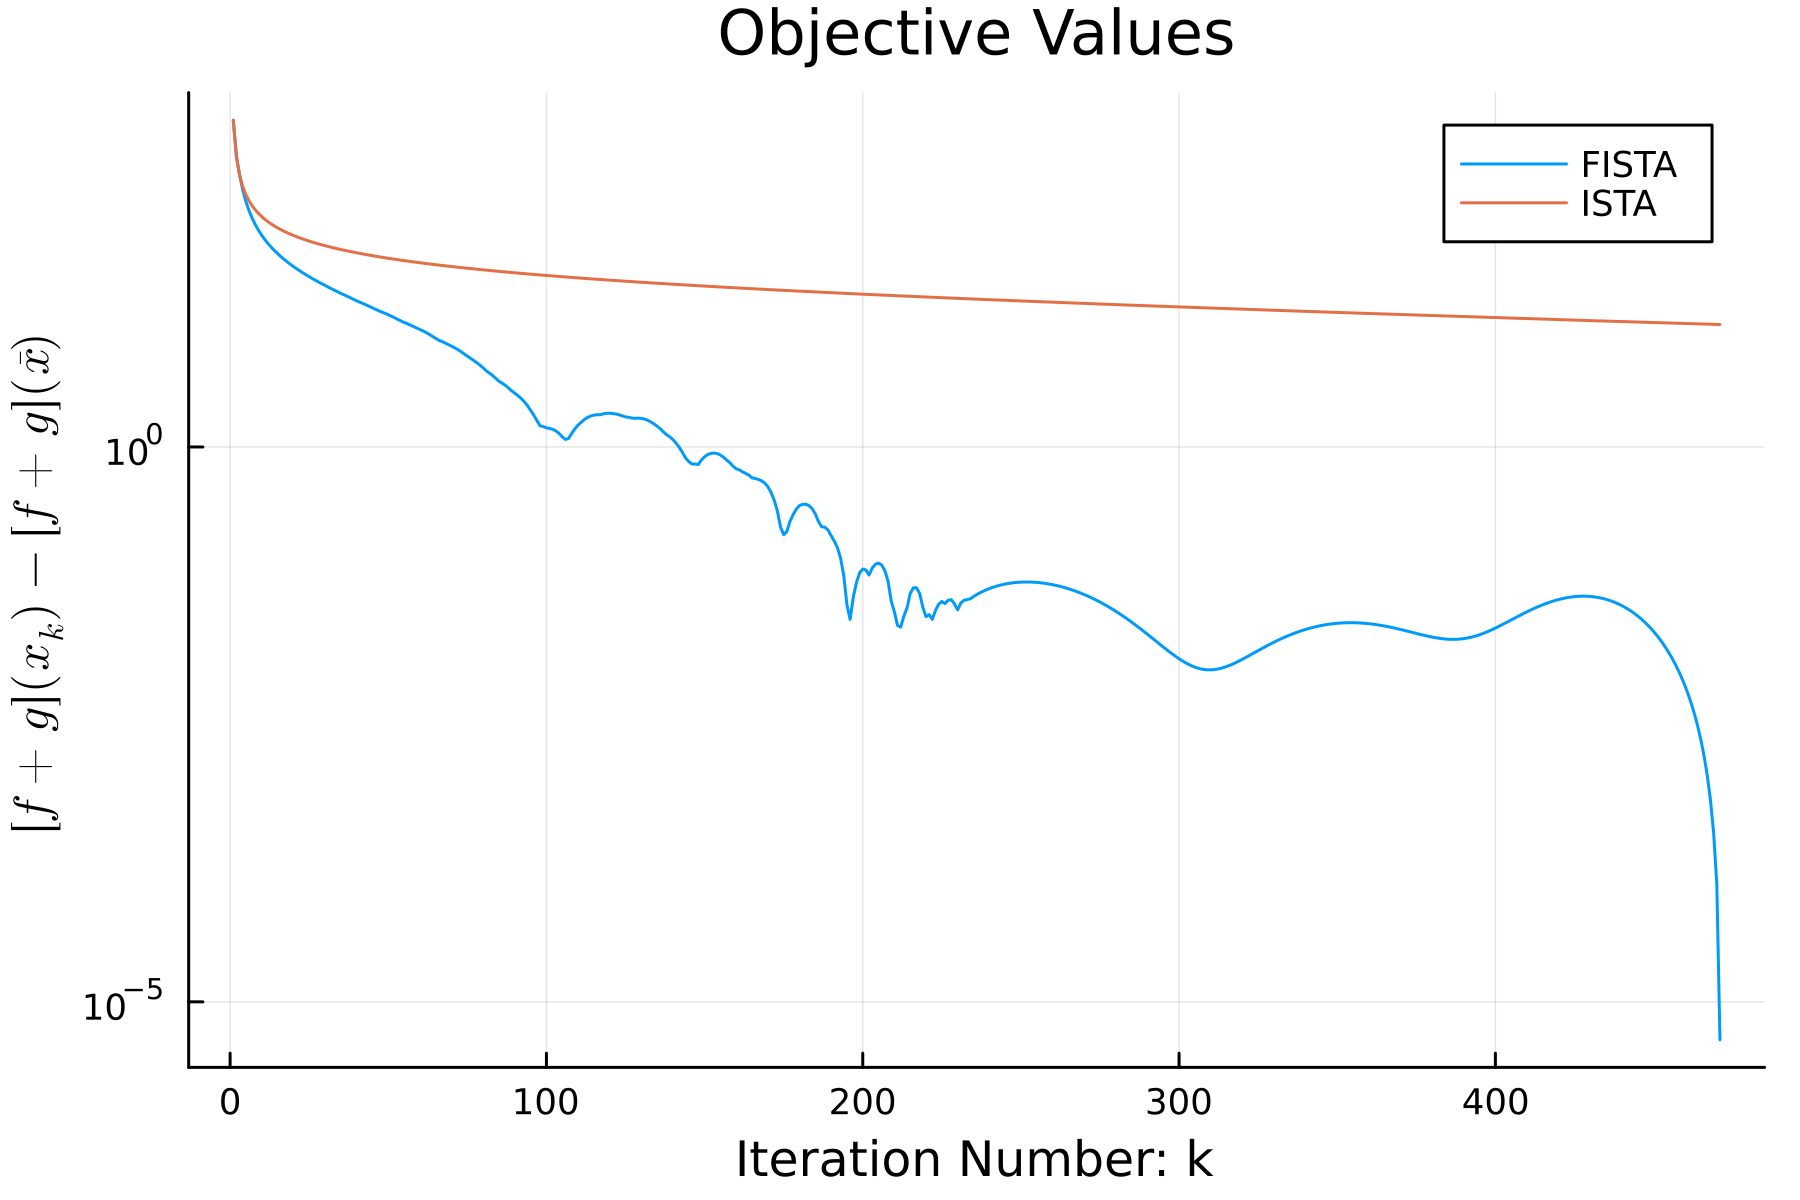
\includegraphics[width=8cm]{Assets/simple_lass_obj.png}
        \caption{The left is the objective value of the function during all iterations.}
    \end{figure}
\end{frame}

\begin{frame}{Results}
    The plot of $\Vert y^{(k)} - x^{(k + 1)}\Vert_\infty$:
    \begin{figure}[h]
        \centering
        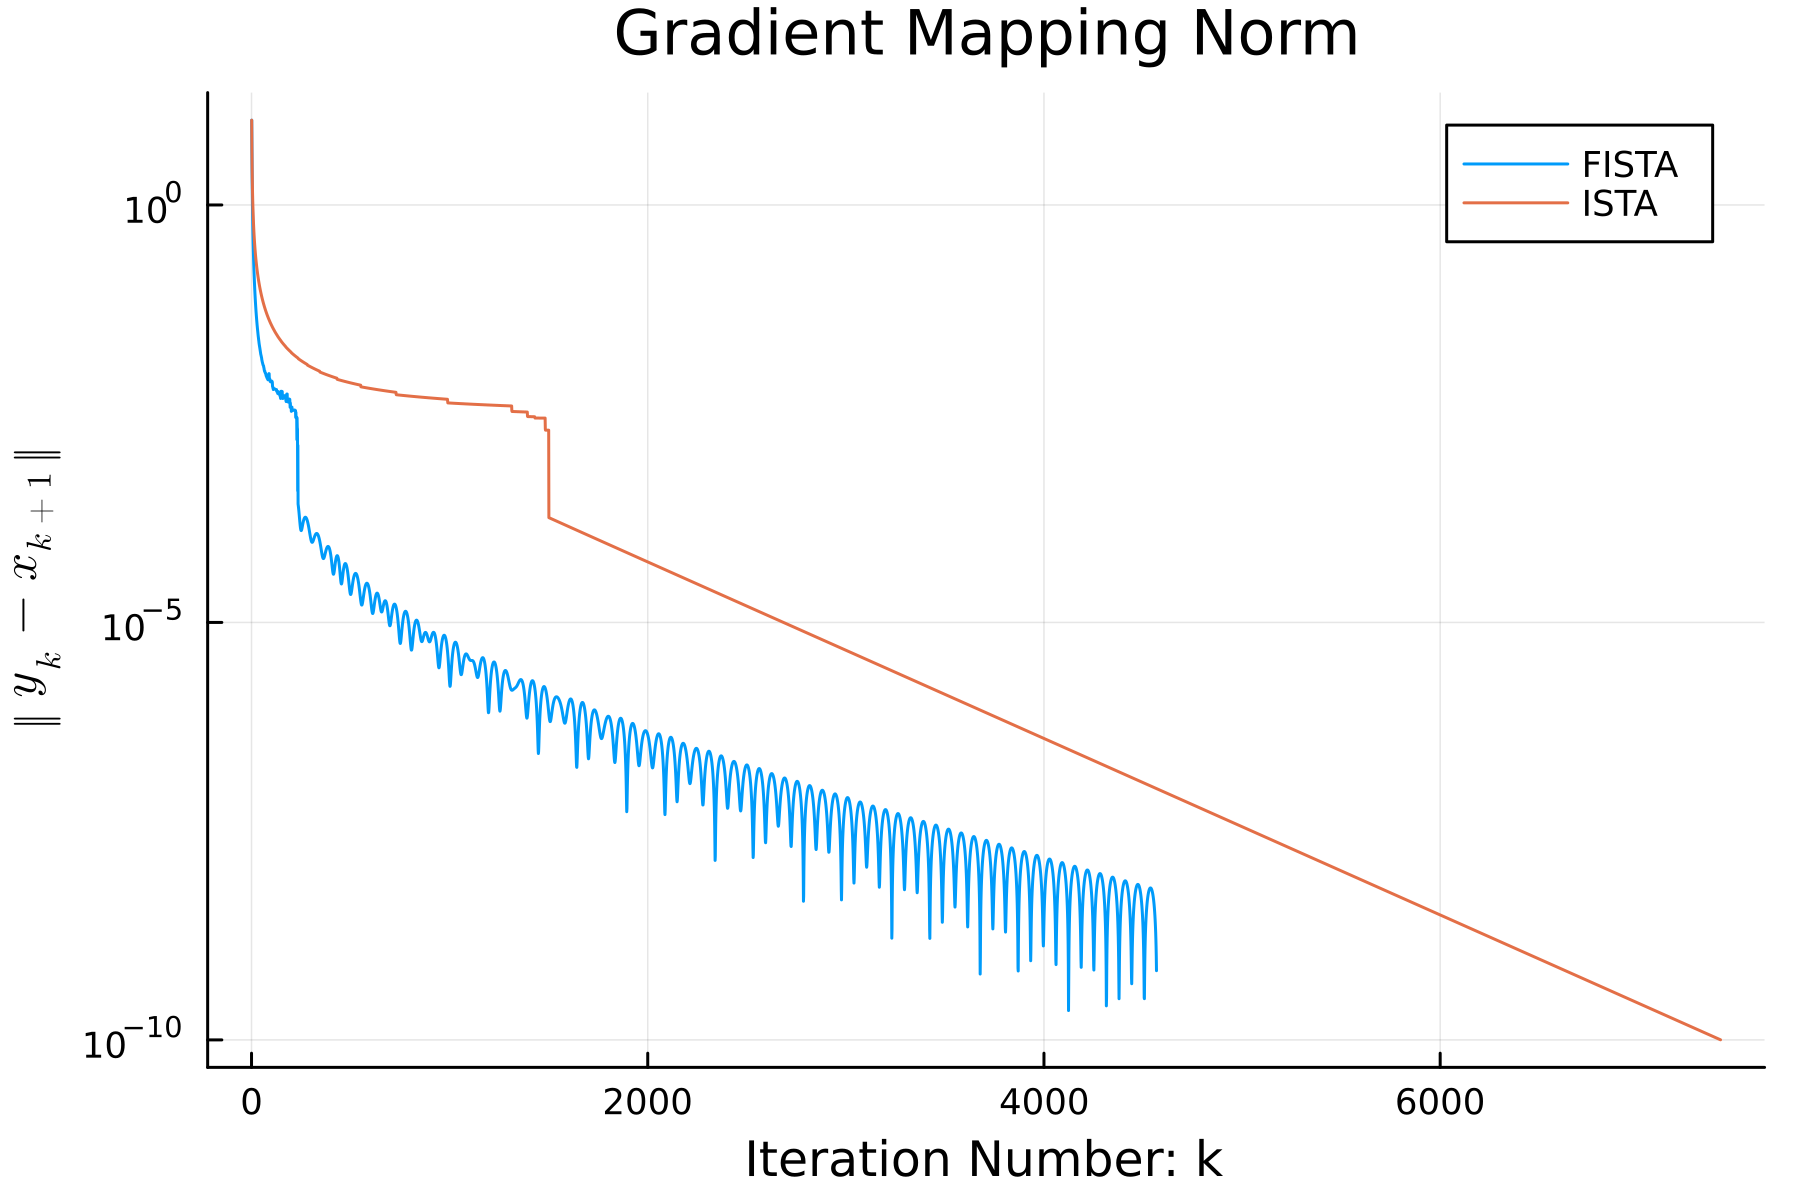
\includegraphics[width=8cm]{Assets/simple_lass_pgrad.png}
    \end{figure}
\end{frame}

\subsection{Image Deconvolution with Noise}
\begin{frame}{Experiment Setup}
    Given an image that is convoluted by a Guassian kernel with some guassian noise, we want to recover the image, given the parameters for convolutions. 
    \begin{itemize}
        \item [1.] Guassian blur with a discrete 15 by 15 kernel is a linear transform represented by a sparse matrix $A$ in the computer. 
        \item [2.] When an image is 500 by 500 with 3 color channels, $A$ is $750000 \times 750000$. 
        \item [3.] Let the noise be on all normalized colors values with $N(0, 10^{-2})$
        \item [4.] We let $\lambda = \alpha\times (3\times500^2)^{-1}$. 
        \item [5.] Implemented in Julia, and the code is too long to be shown here. 
    \end{itemize}        
\end{frame}
\begin{frame}{One Big Image for Some Fancy Results}
    We consider blurring the image of a pink unicorn that I own. 
    \begin{figure}[H]
        \centering
        
\includegraphics[width=5cm]{Assets/blurred_img.jpg}
        \caption{The image is blurred by the Gaussian Blurred matrix $A$ with a tiny amount of noise on the level of $2\times 10^{-2}$ that is barely observable. Zoom in to observe the tiny amount of Gaussian noise on top of the blur.}
        \label{fig:blurred_alto}
    \end{figure}
\end{frame}
\begin{frame}{Moer Image to Show Impressive Results}
    \begin{figure}
        \subfloat[Graph 1]{
            
\includegraphics[width=3cm]{Assets/inverse_linear_experiment1-soln_img.jpg}
            \label{fig:1a}
        }
        \subfloat[Graph 2]
        {
            
\includegraphics[width=3cm]{Assets/inverse_linear_experiment2-soln_img.jpg}
            \label{fig:1b}
        }
        \subfloat[Graph 3]
        {
            
\includegraphics[width=3cm]{Assets/inverse_linear_experiment3-soln_img.jpg}
            \label{fig:1c}
        }
        \caption{(a) $\alpha = 0$, without any one norm penalty, is not robust to the additional noise. (b) $\alpha = 0.01$, there is a tiny amount of $\lambda$. (c) $\alpha = 0.1$, it is more penalty compared to (a).}
        \label{fig:alto_deblurred}
    \end{figure}

\end{frame}
        
    
\section{References}
    \begin{frame}{References}
        
        \bibliography{refs.bib}
    \end{frame}

\end{document}